% Actual stochastic sampling; separate from the older SCFT continuation.
% Generated from positive sampling analysis.json
\newcommand{\SamplingZeroHeight}{$58.56\pm0.35$}
\newcommand{\SamplingTinySigma}{2.67}
\newcommand{\SamplingRhatMax}{1.039}
\newcommand{\SamplingEssMin}{10.1}
\newcommand{\SamplingEssMax}{79.4}
\newcommand{\SamplingPairSigmaMax}{2.42}
\newcommand{\SamplingMaxChargeError}{$2.98e-12$}
\newcommand{\SamplingBathRelativeSe}{0.941}
\newcommand{\SamplingHeightRows}{%
$0.001$ & $57.52\pm0.36$ & $54.31\pm0.22$ & $50.21\pm0.29$ \\
$0.01$ & $54.63\pm0.26$ & $46.02\pm0.21$ & $39.28\pm0.35$ \\
$0.1$ & $43.88\pm0.17$ & $33.04\pm0.19$ & $28.60\pm0.33$ \\
$1$ & $28.49\pm0.21$ & $24.86\pm0.17$ & $23.80\pm0.19$ \\
$10$ & $23.57\pm0.14$ & $23.05\pm0.17$ & $22.80\pm0.29$ \\
}
\newcommand{\SamplingCheckRows}{%
Standard & $400$ & $40$ & $39.28\pm0.35$ \\
Finer grid & $800$ & $40$ & $39.18\pm0.20$ \\
Smaller area & $400$ & $20$ & $37.85\pm0.49$ \\
Larger area & $400$ & $80$ & $39.63\pm0.19$ \\
Salt-free, finer grid & $800$ & $40$ & $58.79\pm0.50$ \\
}
\newcommand{\SamplingControlSigma}{1.63}

\pagetitle{N=100 brush: Monte Carlo sampling}{positivesampling}
\smallnote{2026-09-07\quad /\quad New stochastic calculations, separate from the earlier Fig.~2--3 SCFT scan}

Sample averages were obtained by stochastic updates of incompressible P/S and ion configurations
and the real field in the attractive channel. Parameters were $N=100$, $b=1\units{nm}$,
$\sigma=0.1\units{nm^{-2}}$, $v=1\units{nm^3}$, $\chi=0.5$,
$\ell_B=0.7\units{nm}$, and $a=0.25\units{nm}$.

\textbf{Scope:} a finite planar model retaining only $z$, with 4 chains in $A=40\units{nm^2}$,
$L=200\units{nm}$, and $M=400$ cells. Transverse charge fluctuations are excluded,
so this differs from the paper's 3D statistical model. No LDA self-energy or PB/SCFT solution was inserted into the samples.

\begin{center}
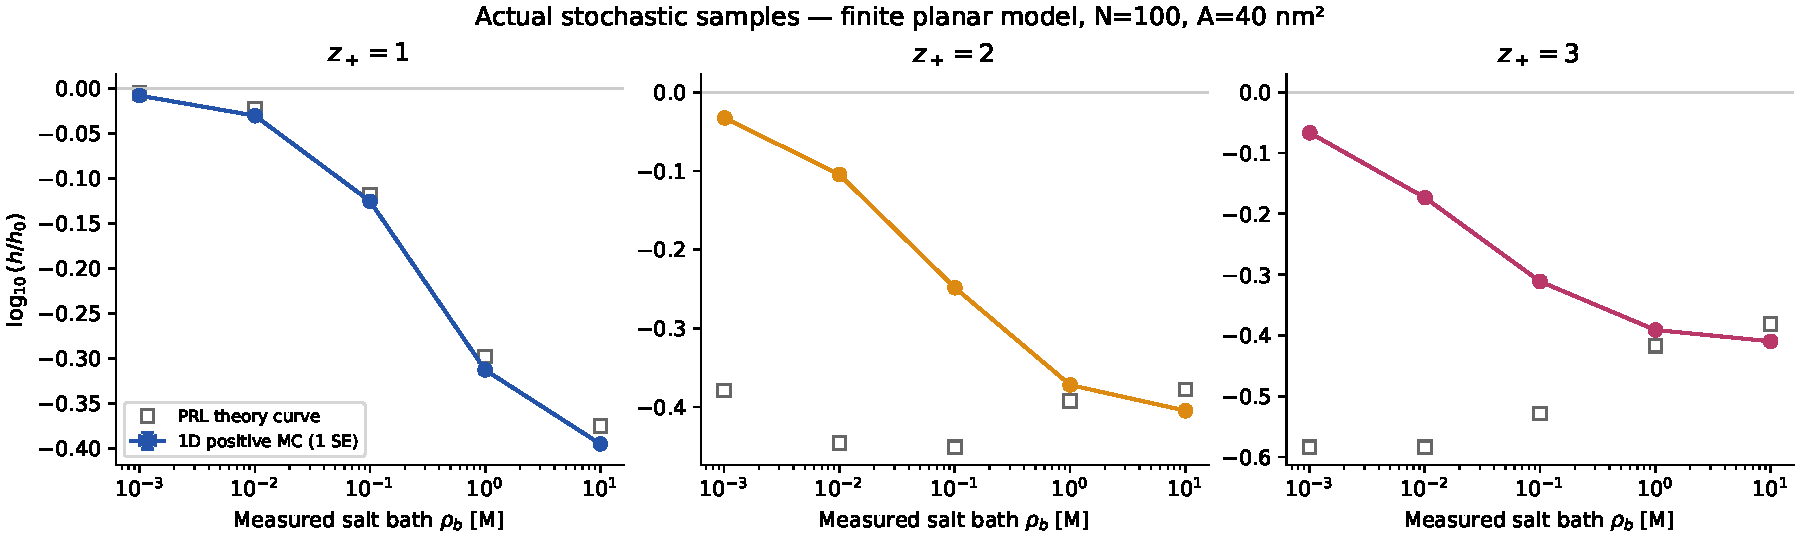
\includegraphics[width=\linewidth]{prl_comparison_figs/positive_brush_20260907/sampling_fig2.pdf}
\end{center}
\vspace{-6pt}
\smallnote{Circles and error bars: sample means and 1 SE. Open squares: digitized PRL theory curves.
The horizontal axis uses concentrations measured in separate pure-salt bulk simulations. The table lists nominal targets.}

\begin{tabularx}{\linewidth}{@{}Xrrr@{}}
\toprule
\rowcolor{panel}Target $\rho_b$ [M] & $z_+=1$: $h$ [nm] & $z_+=2$: $h$ [nm] & $z_+=3$: $h$ [nm] \\
\midrule
\SamplingHeightRows
\bottomrule
\end{tabularx}

\begin{equation*}
 h=\frac{2\int z\langle\rho_P(z)\rangle\,dz}{\sigma N}.
\end{equation*}
\smallnote{The salt-free reference was also sampled directly: $h_0=$\SamplingZeroHeight\,nm.
Height is explicitly defined by the first moment;
it is not automatically equivalent to the paper's Gibbs dividing-surface procedure.
Height decreases at the sampled concentrations, without reproducing the paper's pronounced re-expansion.}

\clearpage
\pagetitle{Sampled distribution and validation}{positivemeasure}
The cell capacity is $K=A\Delta z/v=20$. Polymer paths retain labeled bead coordinates;
solvent is eliminated exactly through $s_j=K-p_j$. Monovalent counterions are fixed at
$\sum_j c_j=n_{\rm chain}N=400$, while salt satisfies $\sum_j n_{-,j}=z_+\sum_j n_{+,j}$.
\begin{align*}
 \pi&\propto B(\bm R)\exp[-U_e-U_\chi]
 \prod_j\frac{a_+^{n_{+,j}}a_-^{n_{-,j}}}{s_j!\,c_j!\,n_{+,j}!\,n_{-,j}!},\\
 U_\chi&=\frac{\chi}{K}\sum_j p_j(K-p_j),\qquad
 U_e=\frac{2\pi\ell_B\Delta z}{A}\sum_e Q_e^2,\\
 Q_e&=\sum_jF_{ej}[-p_j+c_j+z_+n_{+,j}-n_{-,j}].
\end{align*}
$B$ is the weight of Gaussian bonds and a graft source of width $0.5\units{nm}$.
$F_{ej}$ is the cumulative distribution of Gaussian charge of width $a/\sqrt\pi$. The Gaussian
electrostatic field is integrated exactly, including finite-grid self terms. Walls use Neumann electric boundary conditions;
periodic bulk calculations replace $Q_e$ by $Q_e-\overline Q$.

\subhead{Real fields are drawn from their conditional distribution}
\begin{align*}
 e^{(\chi/K)\sum_j(p_j-\bar p)^2}
 &\propto\int_{\sum_jx_j=0}d\bm x\,
 e^{-K\sum_jx_j^2/(4\chi)+\sum_jp_jx_j},\\
 \bm x\mid\bm p&\sim\mathcal N\!\left(
 \frac{2\chi}{K}(\bm p-\bar p),\frac{2\chi}{K}
 \left[I-\frac{\bm1\bm1^T}{M}\right]\right).
\end{align*}
Particle positions use Metropolis updates; ions use binomial conditional redistribution proposals;
salt counts use neutral-cluster insertion and deletion. Same-cell and separated-cell proposals are mixed,
including each reverse proposal probability. Bulk chemical potentials are adjusted only during warmup
and held fixed during measurement and brush sampling. The largest relative bulk concentration SE is \SamplingBathRelativeSe\%.

\subhead{Validation and statistical scope}
Polymer paths, canonical C, and neutral salt configurations were summed directly for 2 cells and 2 beads.
The relative partition error bound from truncating salt counts is below $3\times10^{-40}$.
Across 12 runs ($z_+=1,2,3$, two methods, two seeds), all checked means were within
\SamplingTinySigma\ SE of exact values. Detailed balance and energy updates were checked against independent full weights.

Each of 32 standard brush runs, 2 particle-only controls, and 8 grid/area controls used 200,000 warmup sweeps
and 1,000,000 measurement sweeps. For divalent salt at $0.01\units{M}$, initial split-$\widehat R=1.095$ and
relaxation from the compact start motivated 1,000,000 extra sweeps for both seeds; the table uses these extensions.
The original intervals are preserved. Each sweep includes one random single-bead proposal per bead on average.
Errors account for autocorrelation and 10/20/40-block analysis. Per-run height ESS ranges from
\SamplingEssMin\ to \SamplingEssMax. The maximum split-$\widehat R$ across standard pairs is
\SamplingRhatMax; the largest height difference from particle-only controls is \SamplingControlSigma\ SE.
\textbf{Update counts are not independent sample counts.}

\clearpage
\pagetitle{Fig. 3 from sample averages}{positivefigthree}
\begin{center}
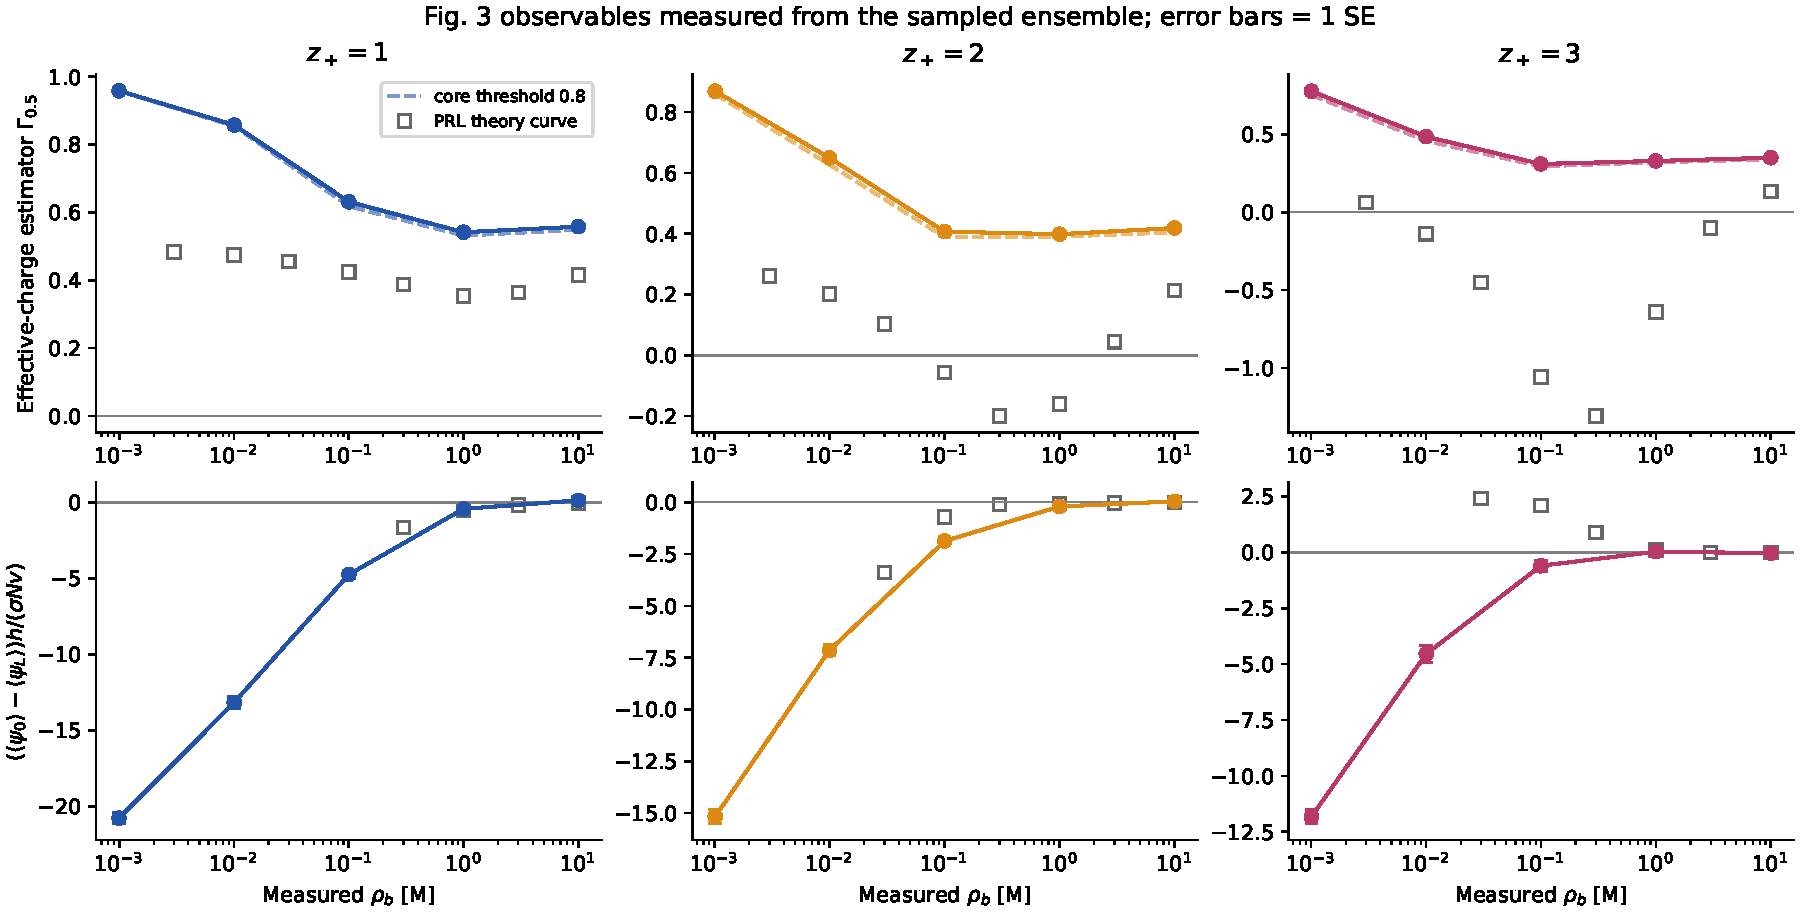
\includegraphics[width=\linewidth]{prl_comparison_figs/positive_brush_20260907/sampling_fig3.pdf}
\end{center}
\vspace{-7pt}
\smallnote{Solid: MC means with core threshold 0.5. Dotted: threshold 0.8. Open squares: PRL theory curves.
Surface potential uses the mean difference between first/last cell centers, without rescaling to fit the paper.}
\begin{align*}
 \overline\Gamma_c&=1-z_+
 \frac{\int_{\langle\rho_P\rangle>c\max\langle\rho_P\rangle}
       [\langle\rho_+\rangle-\rho_b]\,dz}
      {\int_{\langle\rho_P\rangle>c\max\langle\rho_P\rangle}
       \langle\rho_P\rangle\,dz},\\
 \Psi_{\rm rel}&=[\langle\psi(0)\rangle-\langle\psi(L)\rangle]
                  \frac{h}{\sigma Nv}.
\end{align*}
Observables are computed from mean profiles, rather than averaging nonlinear snapshot ratios.
Error estimates include recomputed core boundaries, shared bath uncertainty, and potential--height covariance.
$\Gamma$ differs from the actual net charge including C and anions, which is stored separately in the raw data.

\subhead{Finite-grid and cross-sectional-area controls}
Except for the salt-free row, $z_+=3$ and the target is $\rho_b=0.01\units{M}$.
Chain counts were adjusted with area to retain $\sigma=0.1\units{nm^{-2}}$.
Bulk activities were determined independently for each case.

\begin{tabularx}{\linewidth}{@{}Xrrr@{}}
\toprule
\rowcolor{panel}Control & $M$ & $A$ [nm$^2$] & $h$ [nm] \\
\midrule
\SamplingCheckRows
\bottomrule
\end{tabularx}

For all three valences, $\overline\Gamma_{0.5}$ was positive; potentials at $10\units{M}$ were within 2 SE of zero.
\textbf{Limits:} $A$ sets fluctuation strength in this 1D model, so varying area is more than
a numerical precision check. A few grid controls do not establish continuum convergence.
This restricted model has not reproduced the paper's contraction, re-expansion, and charge/potential reversal
from 3D charge correlations. These results also do not validate convergence of the original CL-FTS dynamics.
\smallnote{Code: \texttt{positive\_brush\_1d.py}, \texttt{run\_positive\_brush.py}.
Numbers, samples, and jobs: \texttt{dh\_salt\_runs/positive\_brush\_20260907/}.
Production FFT/C++/CUDA and the existing CL drift were unchanged in this work.
The following pages retain the earlier small-system and SCFT validation records.}
